\documentclass[PICOReport.tex]{subfiles}

\begin{document}


PICO was designed to respond to requirements posed by the 7 \ac{SOs} listed in Table~\ref{tab:STM}. It will also generate a rich catalog of hundreds of thousands of new sources consisting of proto-clusters, strongly lensed galaxies, and polarized radio and dusty galaxies. An abundance of information about galaxy and cluster evolution, dark matter, the physics of jets of active galactic nuclei, and magnetic fields of dusty galaxies will be stored in this catalog (Table~\ref{tab:STM2}). This catalog will be mined in future years through subsequent analysis and follow-up observations. 
%Here we focus on two specific science deliverables that are enriched by PICO's unique capabilities. %catalog. \comor{Explain Why?}

%\comor{Kathy Romer says: Table 2 - I like the way this is broken down with ?Current knowledge? summaries. But it only talks about Planck. What about ACT, SPT, SO, balloons etc.? Gianfranco: SPT and ACT are already mentioned in connection to strongly lensed galaxies. So far there is not much from them, in the published literature, on source polarization. On proto-clusters there is the recent discovery of one at z=4.3 (Miller et al. 2018). Perhaps we could add that. }

\subsubsection{Early phases of galaxy evolution}

%\comor{Kathy Romer: Section 2.3.1 - page 22 - I noted ?why do we care about lensed high-z galaxies? in the margin. So maybe you need to stress the motivation for this section more? Gianfranco: It is already said that strong lensing provides a unique possibility to look into the structure and kinematics of high-z dusty star-forming galaxies, i.e. to get crucial information on how they form and evolve. I don?t know what to say more.}

PICO's catalog of high-$z$ strongly-lensed galaxies will provide answers to major, still open issues in galaxy formation and evolution. What are the main physical mechanisms shaping the properties of galaxies~\citep{SilkMamon2012, SomervilleDave2015}: in situ processes, interactions, mergers, or cold flows  from the intergalactic medium? And how do feedback processes work? To settle these issues we need direct information on the structure and dynamics of high-$z$ galaxies. But these are compact, with typical sizes of 1--2~kpc~\cite{Fujimoto2018}), corresponding to angular sizes of 0.1--0.2~arcsec at $z\simeq 2$--3. Thus they are hardly resolved, even by ALMA or by HST. If they {\it are} resolved, high enough \ac{SNR}s per resolution element are only achieved for the brightest galaxies, which are probably not representative of the general population.
\begin{figure*}[h]
%\vskip-3cm
\begin{center}
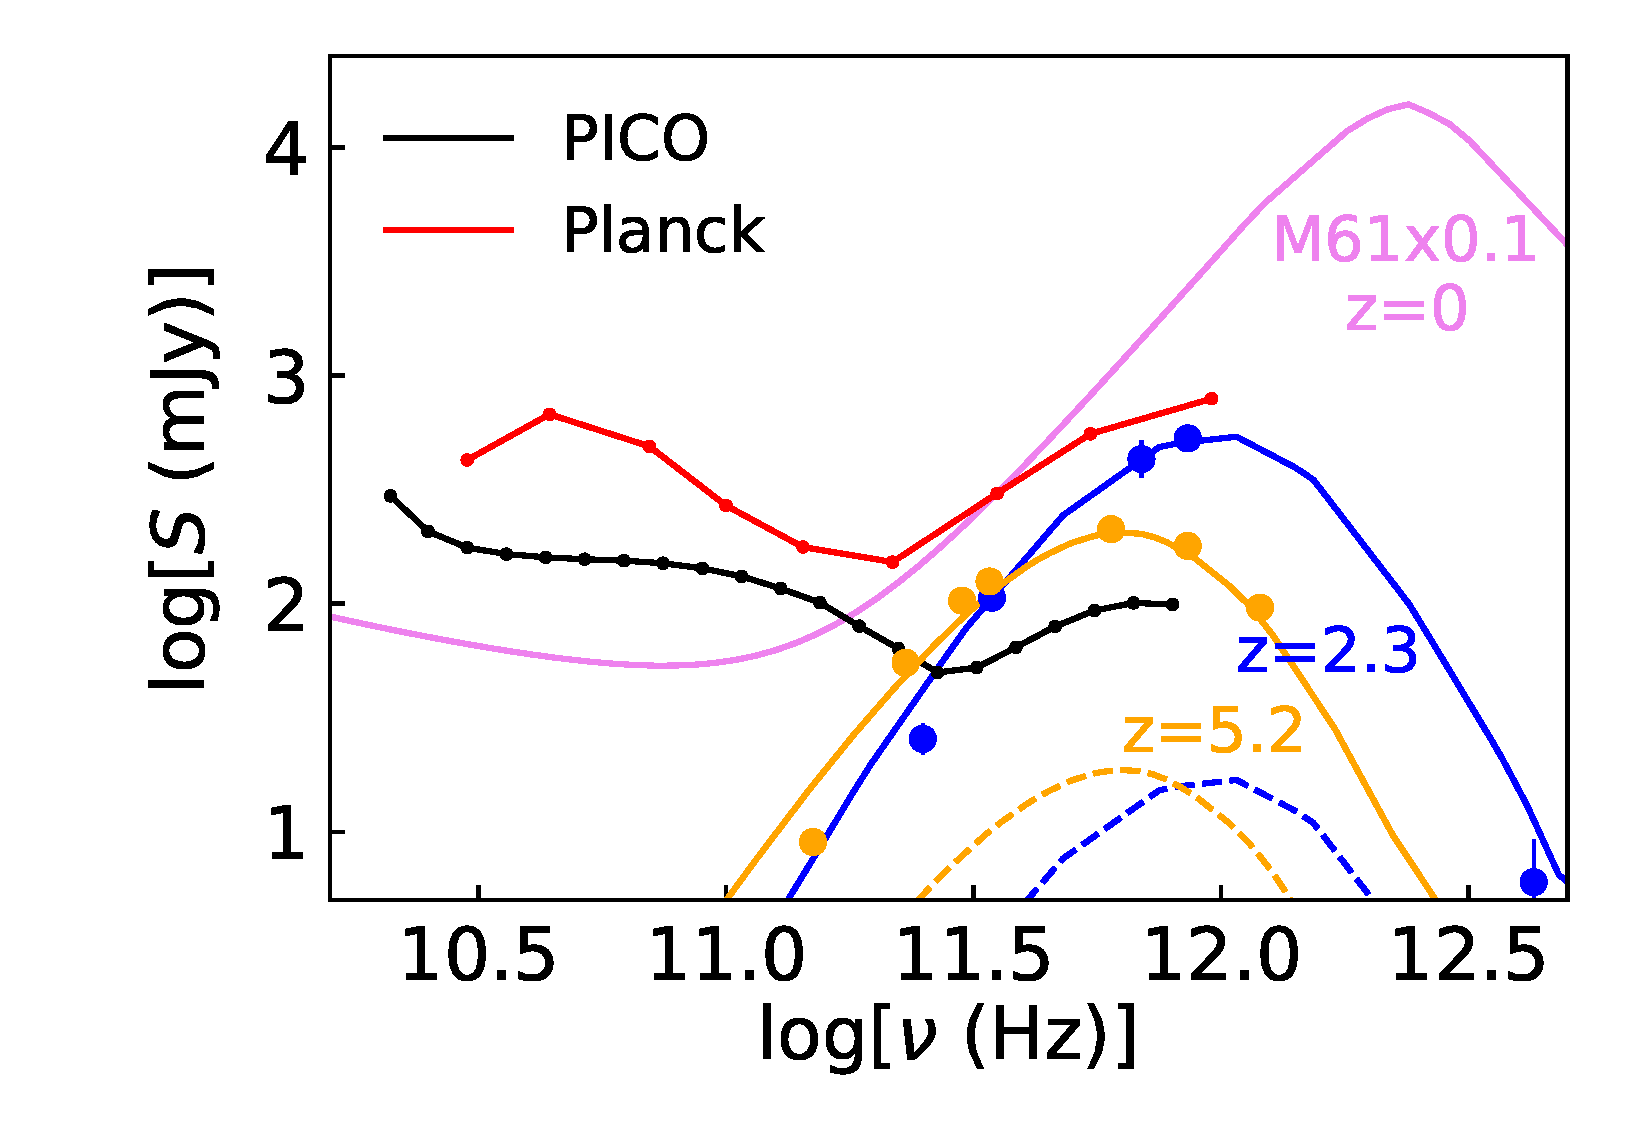
\includegraphics[width=0.416\columnwidth, trim={0 0 0 0cm}, clip]{images/fig_SED_PICO.pdf}
\hspace{0.75cm}
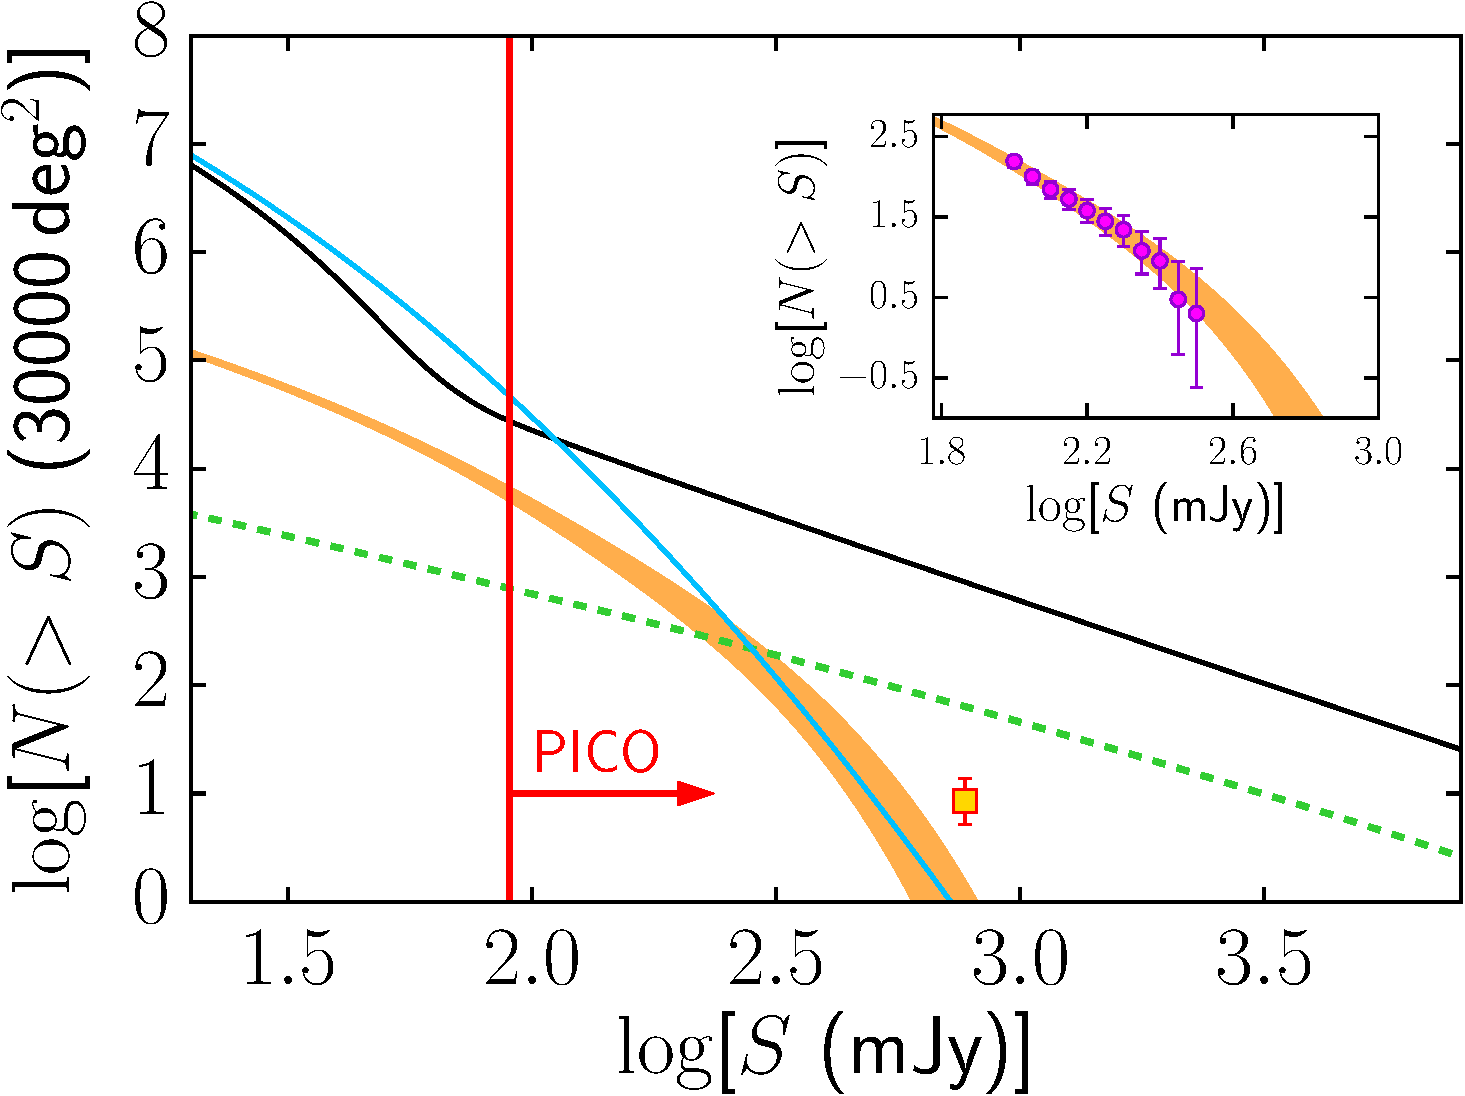
\includegraphics[width=0.4\columnwidth, trim={0 0 0 0cm}, clip]{images/NgtF_pico_NEWNEW.pdf}
\vskip-0.3cm
\caption{ \captiontext {\bf Left:} PICO will detect thousands of new strongly lensed galaxies near the peak of their spectral energy distributions (SEDs), such as SMM\,J2133-0102 (blue)  at $z=2.3$~\cite{Swinbank2010} and HLSJ$091828.6{+}514223$ (orange) at $z=5.2$~\cite{Combes2012}. The dashed lines are the SEDs pre-lensing-induced magnification. PICO's higher resolution gives point-source detection limits (black line) that are up to 10 times fainter compared to \planck 's 90\% completeness limits (red line~\cite{PCCS2}). High frequency measurements ($\nu>300$~GHz) of 30,000 low-z galaxies, like M61 (magenta, SED was scaled down by a factor of ten.), will give a census of their cold dust.  {\bf Right panel.} Integral counts of unlensed (black) and strongly lensed, high-$z$ (orange) star-forming galaxies for 70\% of the sky away from the Galactic plane at 600~GHz based on fits of \textit{Herschel} counts over 1000 deg$^2$ (inset~\citep{Negrello2017lensed}). The PICO detection region (right of vertical red line) will yield a factor of 1000 increase in strongly lensed galaxies relative to \planck~(yellow square), as well as about 50,000 proto-clusters (blue) and 2,000 radio sources (green)~\citep{Negrello2017protocl}. }
%Also shown are predicted radio source counts (green). }
\label{fig:SED3}
\end{center}
\vspace{-0.15in}
\end{figure*}

Strong gravitational lensing provides a solution to these problems. Since lensing conserves the surface brightness, the effective angular size is stretched on average by a factor of $\mu^{1/2}$, where $\mu$ is the gravitational magnification, thus substantially increasing the resolving power. A spectacular example is ALMA observations of the \planck-discovered, strongly lensed galaxy PLCK\_G244.8\-+54.9 at $z \simeq 3.0$  with $\mu \simeq 30$~\citep{Canameras2017ALMA}. ALMA observations with a $0.1''$ resolution reached an astounding spatial resolution of 60~pc, substantially smaller than the size of a Milky Way giant molecular clouds. CO spectroscopy of this object, measuring the kinematics of the molecular gas, gave an uncertainty of 40--50~km/s. Such precision allows a high \ac{SNR} detection of the predicted $\sim 1000\,\hbox{km}\,\hbox{s}^{-1}$  outflows capable of sweeping the galaxy clear of gas that would otherwise be available for star formation~\citep{KingPounds2015}. In this specific case, there were no clear indications that mergers or cold flows shaped the galaxy, but similar spectroscopy of another strongly lensed galaxy at $z=5.3$ detected a fast (800 km/s) molecular outflow due to feedback. 
%The outflow carries mass at a rate close to the star-formation rate, and can thus remove a large fraction of the gas that would otherwise be available for star formation.  
% Ca\~{n}ameras et al.~\citep{Canameras2017ALMA} have obtained CO spectroscopy for this object, measuring the kinematics of the molecular gas with an uncertainty of 40--50~km/s. This spectral resolution makes possible a direct investigation of massive outflows driven by AGN feedback at high $z$. Using this technique \citet{Spilker2018} detected a fast (800 km/s) molecular outflow due to feedback in a strongly lensed galaxy at $z=5.3$. They found that the outflow carries mass at a rate close to the star formation rate, and can thus remove a large fraction of the gas that would otherwise be available for star formation.

PICO will detect thousands of early forming galaxies whose flux densities are boosted by large factors (Fig.~\ref{fig:SED3}, right).
Currently there are reports of just a few other high-$z$ galaxies that are spatially resolved thanks to gravitational lensing, albeit with less extreme magnifications~\citep{Dye2018, Lamarche2018, Sharda2018}. PICO's catalog will be transformative as it will probe the \ac{SED} of the lensed galaxies at their peaks. Two examples of known sources are shown in the left panel of Figure~\ref{fig:SED3}. While ground-based instruments observe at frequencies up to $\log \nu = 11.45$, PICO's data will extend to the peak of the \ac{SED}, up to $\log \nu = 11.9$ (Fig.~\ref{fig:SED3}, left).

A straightforward extrapolation of the \textit{Herschel} counts to the 70\% non-Galactic sky gives a detection of 4,500 strongly-lensed galaxies with a redshift distribution peaking at $2\simlt z \simlt 3$~\cite{Negrello2017lensed}, but extending up to $z> 5$ (Fig.~\ref{fig:SED3}, left panel).\footnote{Extrapolating from achieved performance by the South Pole Telescope~\cite{??}, we estimate that S3 experiments will detect $\sim$1,600 such sources, and only in the RJ part of the spectrum.} If objects like the $z=5.2$ strongly lensed galaxy HLSJ091828.6+514223 exist at higher redshifts, they will be detectable by PICO out to $z>10$. At the 600~GHz detection limit, about 25\% of all detected extragalactic sources will be strongly lensed; for comparison, at optical/near-IR and radio wavelengths, where intensive searches have been carried out for many years, the yield is only about 0.1\%, that is more than two orders of magnitude lower~\cite{Treu2010}. To add to the extraordinary sub-mm lensing bonanza, the selection of PICO-detected strongly lensed galaxies will be extremely easy because of their peculiar sub-mm colors (Fig.~\ref{fig:SED3}, left panel), resulting in a selection efficiency close to 100\% \citep{Negrello2010}. The survey will give the brightest objects over the entire sky, maximizing the efficiency of selecting sources for follow-up observations. 
%\comor{need to compare to SO, extrapolated from SPT}

The intensive high spectral and spatial resolution follow-up campaign of this large sample will enable a leap forward in our understanding of the processes driving early galaxy evolution and open up other exciting prospects, both on the astrophysical and on the cosmological side (see for example~\citet{Treu2010}).

\subsubsection{Early phases of cluster evolution}

PICO will open a new window for the investigation of early phases of cluster evolution, when their member galaxies were actively star forming (and dusty), but the hot \ac{IGM} was not necessarily in place. In this phase, traditional approaches to cluster detection (X-ray and SZ surveys, and searches for galaxy red sequences) work only for the more evolved clusters, which do include hot \ac{IGM}; indeed these methods have yielded only a handful of confirmed proto-clusters at $z\simgt 1.5$ \cite{Overzier2016}.\footnote{More high-$z$ proto-clusters have been found by targeting the environment of tracers of very massive halos, such as radio-galaxies, QSOs, sub-mm galaxies. These searches are, however, obviously biased.} \planck~has demonstrated the power of low-resolution surveys for the study of large-scale structure~\cite{Planck2016high_z}, but its resolution was too poor to detect individual proto-clusters \cite{Negrello2017protocl}.  Studies of the high-$z$ 2-point correlation function \cite{Chen2016, Negrello2017protocl} and \textit{Herschel} images of the few sub-mm bright protoclusters detected so far, at $z$ of up to 4 \cite{Ivison2013, Wang2016, Oteo2018}, all of which will be detected by PICO, indicate sizes of $\simeq 1'$ for the proto-cluster cores, nicely matching the PICO FWHM at the highest frequencies.

PICO will detect 50,000 proto-clusters as peaks in the high frequency maps, which are not available for ground-based instruments (Table~\ref{tab:STM2}; blue line in the right-hand panel of Fig.~\ref{fig:SED3}).\footnote{Extrapolating from achieved performance by the South Pole Telescope~\cite{??}, we estimate that S3 experiments will detect few hundred sources.} The redshift distribution will extend out to $z\sim4.5$. This catalog will be augmented by 150,000 evolved clusters, detected by the SZ effect. This will constitute a breakthrough in the observational validation of the formation history of the most massive dark-matter halos, traced by clusters, a crucial test of models for structure formation. Follow-up observations will characterize the properties of member galaxies, probing galaxy evolution in dense environments and shedding light on the complex physical processes driving it.

\subsubsection{Additional products of PICO surveys}

PICO will yield a complete census of cold ($<20$K) dust, available to sustain star formation in the nearby Universe, by detecting tens of thousands of galaxies mostly at $z\simlt 0.1$; the \ac{SED} of M61 is a typical example (Fig.~\ref{fig:SED3}, left). With a statistical population, and information only available using data at frequencies above 300~GHz, we will investigate the distribution of such dust as a function of galaxy properties, such as morphology, and stellar mass. 

PICO will increase by an order of magnitude the number of blazars selected at sub-mm wavelengths and will determine the SEDs of many hundreds of them up to 800\,GHz and up to $z> 5$. Blazar searches are the most effective way to sample the most massive black holes at high $z$ because of the Doppler boosting of their flux densities. PICO's surveys of the largely unexplored mm/sub-mm spectral region will also offer the possibility to discover new transient sources or events, such as blazar outbursts~\cite{Metzger2015}.

PICO will make a leap forward in the determination of the polarization properties of both radio sources and of dusty galaxies over a frequency range where ground-based surveys are impractical or impossible. At 320 (800)~GHz it will find 1,200~(500) radio sources and 350~(15,000) dusty galaxies at flux limit down to 4~(6)~mJy.  These data will give information on the structure and ordering of dusty-galaxies' large-scale magnetic fields. In the case of radio sources emission at higher frequencies comes from regions closer to the central engine, providing information on the innermost regions of the jets, close to the active nucleus. 

The anisotropy of the \ac{CIB}, produced by dusty star-forming galaxies over a wide redshift range, is an excellent probe of the history of star formation across time. The \planck\ collaboration derived values of the star-formation rate out to $z\sim4$~\cite{2014A&A...571A..30P,2014A&A...571A..18P,madau2014}). PICO's lower noise and twice the number of frequency bands will give an order of magnitude improvement on the statistical errors for parameters describing the rate of star-formation history~\cite{Wu:2016hej}. Similar improvement will be achieved in constraining $M_{\mathrm{eff}}$, the galaxy halo mass that is most efficient in producing star-formation activity. PICO's increased sensitivity to Galactic dust polarization will enhance the separation of signals coming from the largely unpolarized \ac{CIB} and polarized Galactic dust; an effective separation of signals currently limits making reliable, legacy-quality \ac{CIB} maps. 
By providing a nearly full-sky map of matter fluctuations traced by dusty star-forming galaxies, such a set of maps could be used for delensing the CMB~\cite{Sherwin/Schmittfull}, for measuring local primordial non-Gaussianity from \ac{CIB} auto-correlations~\cite{tucci}, or for cross-correlations with CMB lensing~\cite{Schmittfull/Seljak}.

%By providing a nearly full-sky map of matter fluctuations traced by highly biased galaxies, such a set of maps could be used for delensing the CMB~\cite{Schmittfull/seljak}, or for measuring local primordial non-Gaussianity from \ac{CIB} auto-correlations~\cite{tucci}. 

%The anisotropy of the \ac{CIB}, produced by dusty star-forming galaxies over a wide redshift range, is an excellent probe of both the history of star formation and the link between galaxies and dark matter across time. The \planck\ collaboration derived values of the star-formation rate out to $z\sim4$~\cite{2014A&A...571A..30P,2014A&A...571A..18P,madau2014}). PICO's lower noise and broader frequency coverage will give an order of magnitude improvement on the statistical errors for parameters describing the rate of star-formation history~\cite{Wu:2016hej}. \comor{what are the parameters?} Similar improvement will be achieved in constraining $M_{\mathrm{eff}}$, the galaxy halo mass that is most efficient in producing star-formation activity. PICO's increased sensitivity to Galactic dust polarization will enhance the separation of signals coming from the largely unpolarized \ac{CIB} and polarized Galactic dust; an effective separation of signals currently limits making reliable, legacy-quality \ac{CIB} maps.

%For example, a key parameter in
%simulations of the angular power spectrum of the \ac{CIB}
%is $M_{\mathrm{eff}}$, the galaxy halo mass that is most efficient in producing star
%formation activity. Comparing measurements of the power spectrum to simulations
%constrains this parameter, which informs structure formation models. Current models and measurements
%find $M_{\mathrm{eff}}\sim 10^{12}$ solar masses with about $\mathrm{10\%}$ uncertainty.
%The CMB Probe will constrain this parameter at the percent level.

%Dusty star-forming galaxies trace the underlying dark matter
%field in a broad redshift range. Therefore, a wealth of information will be extracted by
%correlating the anisotropy in the \ac{CIB}
%with multiple dark matter tracers including catalogs of galaxies and quasars,
%and maps of the $\gamma$-ray and the X-ray background~\cite{serra2014,wang2015,cooray2016}.
%These cross-correlations will provide an additional probe of the star formation history, and they will shed light on the interaction between
%light and matter in a broad wavelength range. \comred{the paragraph starts with dark matter, but ends
%with SFR ..?}


\end{document}

%%%%%%%%%%%%%%%%%%%%%%%%%%%%%%%
